\documentclass[]{article}
\usepackage{amsmath}\usepackage{amsfonts}
\usepackage[margin=1in,footskip=0.25in]{geometry}
\usepackage{mathtools}
\usepackage{hyperref}
\hypersetup{
    colorlinks=true,
    linkcolor=blue,
    filecolor=magenta,
    urlcolor=cyan,
}
\usepackage[final]{graphicx}
\usepackage{listings}
\usepackage{courier}


\lstset{basicstyle=\tiny\ttfamily,breaklines=true}

% \usepackage{wrapfig}
\graphicspath{{.}}

\begin{document}
\begin{center}
    Class: AMATH 583\quad Name: Hongda Li \quad HW3 Questions.rst
\end{center}
\section*{Quetion 1}
    What level of SIMD/vector support does the CPU your computer provide?
    \\[1.1em]
    List of SIMD provided by 4900HS:
    \begin{enumerate}
    \item[1.] AVX2, AVX
    \item[2.] SSE, SSE3, SSSE3 SSE4.1, SSE4.2, SSE2 
    \end{enumerate}
    The SSE is just old type of AVX.
    
\section*{Questions 2, 3}
    What is the maximum operand size that your computer will support?
    \\[1.1em]
    AVX2 provides the longest register length for data, in this case it's 256 bit.


\section*{Question 4}
    What is the clock speed of your CPU?  (You may need to look this up via "About this Mac" or "lscpu").
    \\
    Base: 3.0 GHz, Boost: 4.3 GHz, usually I get 3.9GHz. 

\section*{Question 5}
    Based on the output from bandwidth.exe on your computer, what do you expect L1 cache and L2 cache sizes to be?  What are the corresponding bandwidths?   How do the cache sizes compare to what ``about this mac" (or equivalent) tells you about your CPU?  (There is no "right" answer for this question -- but I do want you to do the experiment.)
    \\[1.1em]
    This is the verbatim of the out of from ``./bandwidth.exe'' command: 
    \begin{lstlisting}
        read        
    bytes/elt       #elts   res_bytes   ntrials          usecs      ttl_bytes      bytes/sec
            8          16         128  67108868          15000     8589935104    5.72662e+11
            8          32         256  33554436           8000     8589935616    1.07374e+12
            8          64         512  16777220           4000     8589936640    2.14748e+12
            8         128        1024   8388612           1000     8589938688    8.58994e+12
            8         256        2048   4194308              0     8589942784              0
            8         512        4096   2097156           1000     8589950976    8.58995e+12
            8        1024        8192   1048580              0     8589967360              0
            8        2048       16384    524292              0     8590000128              0
            8        4096       32768    131074              0     4295032832              0
            8        8192       65536     65538              0     4295098368              0
            8       16384      131072     32770              0     4295229440              0
            8       32768      262144     16386              0     4295491584              0
            8       65536      524288      8194              0     4296015872              0
            8      131072     1048576      2049              0     2148532224              0
            8      262144     2097152      1025              0     2149580800              0
            8      524288     4194304       513              0     2151677952              0
            8     1048576     8388608       257              0     2155872256              0
            8     2097152    16777216       129              0     2164260864              0
            8     4194304    33554432        65              0     2181038080              0
            8     8388608    67108864        33              0     2214592512              0
            8    16777216   134217728        17              0     2281701376              0
    write       
    bytes/elt       #elts   res_bytes   ntrials          usecs      ttl_bytes      bytes/sec
            8          16         128  67108868          62000     8589935104    1.38547e+11
            8          32         256  33554436          62000     8589935616    1.38547e+11
            8          64         512  16777220          61000     8589936640    1.40819e+11
            8         128        1024   8388612          61000     8589938688    1.40819e+11
            8         256        2048   4194308          61000     8589942784    1.40819e+11
            8         512        4096   2097156          61000     8589950976    1.40819e+11
            8        1024        8192   1048580          61000     8589967360    1.40819e+11
            8        2048       16384    524292          61000     8590000128     1.4082e+11
            8        4096       32768    131074          32000     4295032832     1.3422e+11
            8        8192       65536     65538          33000     4295098368    1.30154e+11
            8       16384      131072     32770          31000     4295229440    1.38556e+11
            8       32768      262144     16386          31000     4295491584    1.38564e+11
            8       65536      524288      8194          32000     4296015872     1.3425e+11
            8      131072     1048576      2049          22000     2148532224    9.76606e+10
            8      262144     2097152      1025          23000     2149580800      9.346e+10
            8      524288     4194304       513          51000     2151677952    4.21898e+10
            8     1048576     8388608       257         364000     2155872256    5.92273e+09
            8     2097152    16777216       129         351000     2164260864    6.16599e+09
            8     4194304    33554432        65         366000     2181038080    5.95912e+09
            8     8388608    67108864        33         360000     2214592512    6.15165e+09
            8    16777216   134217728        17         375000     2281701376    6.08454e+09
    read/write
    bytes/elt       #elts   res_bytes   ntrials          usecs      ttl_bytes      bytes/sec
            8           8         128  67108868         108000     8589935104    7.95364e+10
            8          16         256  33554436         130000     8589935616    6.60764e+10
            8          32         512  16777220          65000     8589936640    1.32153e+11
            8          64        1024   8388612          44000     8589938688    1.95226e+11
            8         128        2048   4194308          37000     8589942784    2.32161e+11
            8         256        4096   2097156          34000     8589950976    2.52646e+11
            8         512        8192   1048580          32000     8589967360    2.68436e+11
            8        1024       16384    524292          31000     8590000128    2.77097e+11
            8        2048       32768    131074          17000     4295032832    2.52649e+11
            8        4096       65536     65538          32000     4295098368    1.34222e+11
            8        8192      131072     32770          32000     4295229440    1.34226e+11
            8       16384      262144     16386          33000     4295491584    1.30166e+11
            8       32768      524288      8194          33000     4296015872    1.30182e+11
            8       65536     1048576      2049          21000     2148532224    1.02311e+11
            8      131072     2097152      1025          20000     2149580800    1.07479e+11
            8      262144     4194304       513          44000     2151677952    4.89018e+10
            8      524288     8388608       257         265000     2155872256    8.13537e+09
            8     1048576    16777216       129         264000     2164260864    8.19796e+09
            8     2097152    33554432        65         262000     2181038080    8.32457e+09
            8     4194304    67108864        33         265000     2214592512    8.35695e+09
            8     8388608   134217728        17         203000     2281701376    1.12399e+10
    \end{lstlisting}
    The compiler optimized out the read forloop, making the results invalid. I currently don't have a good idea on how to get the read speed yet.
    \\[1.1em]
    For the write, a Plateau appeared between the block size of ``65536'' to ``131072'', indicating a threshold of $2^{16}$ bits for the L1 registers. Which is about ``64kb'' L1 Cache. The second Plateau appeared between size ``524288'' and ``1048576 '' bytes, meaning that L2 could have a size of ``512''kb. The third plateau happens around 8mb, and that could potentially be entering the L3 cache. 
    \\[1.1em]
    For the read/write bandwidth to register, it's a different story. It seems like, for blocks that are too small, it's unable to achieve optimal speed, and the speed drops out,  around ``256kb''. 
    \\[1.1em]
    L1 Cache has speed around ``1.3425e+11''bytes/s, which is about ``134.25 gb/s''. And the decrease L2 speed is about ``90 gb/s'', and for L3, it's about ``6gb/s''. 
    \\[1.1em]
    The specs of the Ryzen 4900HS has 512kb for L1 register, and 4.0mb for L2 Register, and I think L3 is shared between 2 cluster of cores so we are not worrying about that. 
    \\[1.1em]
    Therefore, it seems like there are 2 types of speed for L1 cache for this CPU, I mistaken the first Plateau as falling L1 to L2, but actually it's not. 
    \\[1.1em]
    I googled a bit, and here is the source for \href{https://en.wikichip.org/wiki/amd/ryzen_9/4900hs}{4900HS cache organization}. 
    \\[1.1em]
    For L1, there are 2 types of L1, L1L, L1D, and for L2, it's 512kb shared for one core while 4 ways stitched together for 4 coers. 
    \\[1.1em]
    L3 is 2 times 4 mb (8 mb in total) and between 2 groups of 4 cores. 
    \\[1.1em]
    \textbf{Note}: The Ryzen zen 2 CPU should also have a FMA4 (Fused, Multiply Add) SIMD instruction set for floating operations, however, it's not shown when ``./cpuinfo583.exe'' is executed. 

\section*{Questions 6}
    Based on the output from bandwidth.exe on your computer, what do you expect L1 cache and L2 cache sizes to be?  What are the corresponding bandwidths?   How do the cache sizes compare to what "about this mac" (or equivalent) tells you about your CPU?  (There is no "right" answer for this question -- but I do want you to do the experiment.)
    \\
    \begin{center}
        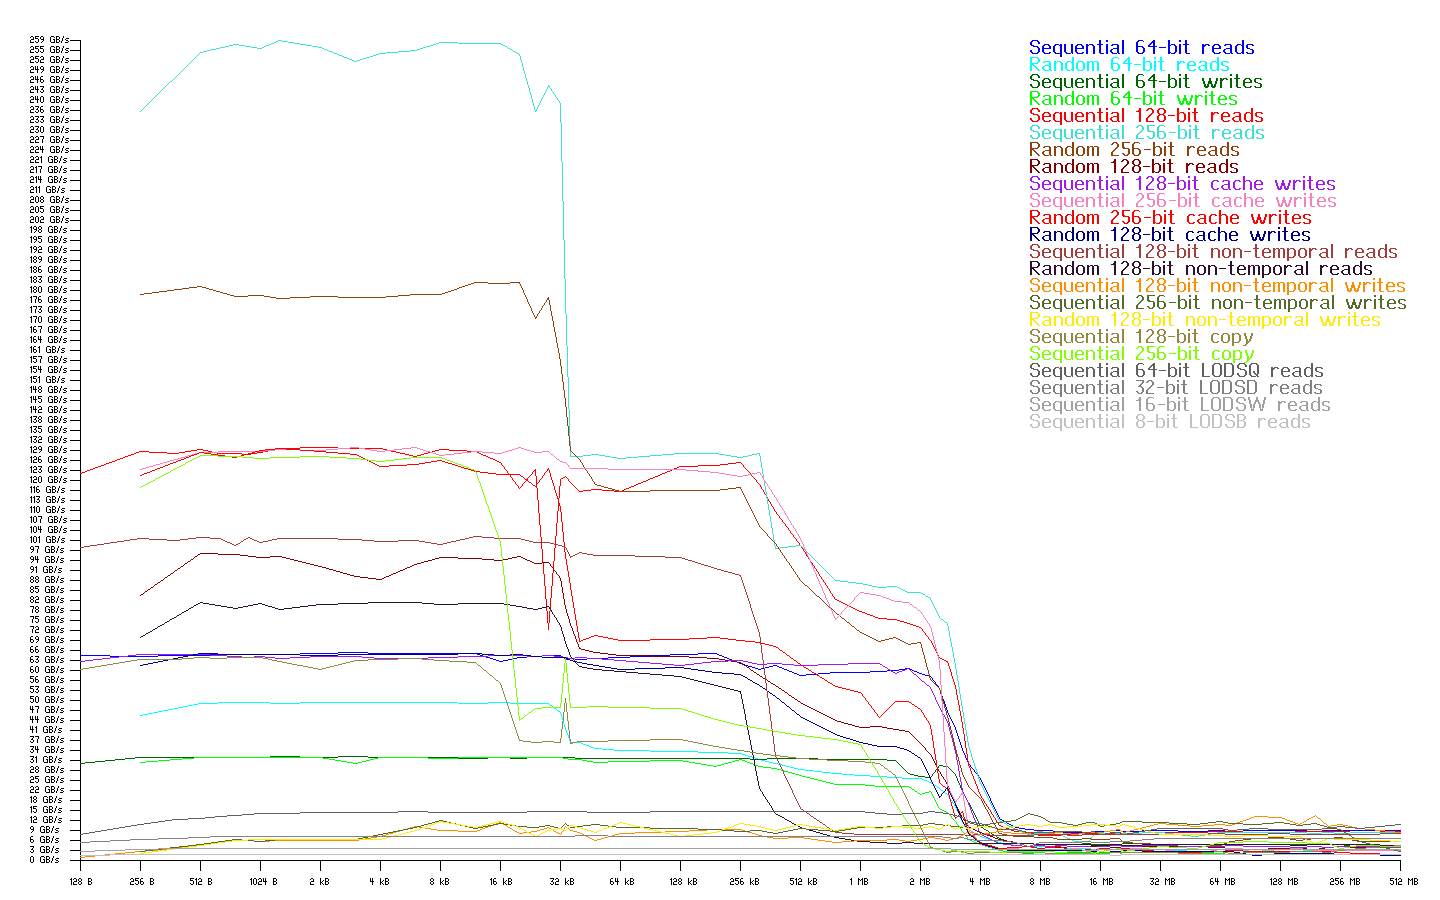
\includegraphics[width=12cm]{bandwidth.png}
    \end{center}
    There are 3 drops in the data bandwidth from the experiment, at the size of 32kb, 512 kb, and 4mb. Each of them corresponds to part of the L1 cache (each core has independent 32kb of cache to work with), all of the L1 cache, L2. And by the time we entered L3 cache (around 4mb), all the speed is gone because we are in the DRAM territory. 
\section*{Question 7}
    What is the (potential) maximum compute performance of your computer?  (The horizontal line.)  What are the L1, L2, and RAM bandwidths?  How do those bandwidths correspond to  what was measured above with the bandwidth program?
    \begin{enumerate}
        \item [1.]
        Assume single core performance, The top speed is computed by: 
        $$
            \text{(Core Speed)} 
            \times 
            \text{(Instruction per clcye)}
            \times
            \text{(Number of Floats it can process with SIMD)}
        $$
        hence the number will be given by: 
        $$
        4.3 \times 8 [\text{GFlops}/s] \approx 34.4 [\text{Gflops}/s]
        $$
        where the data ``8'' is for double precision floating points, using the ``FMA3" instruction for ryzen processor. However, if the ``256'' bits register is used with the ``AVX2'' SIMD, then the data Gflops will be $4.3\times 4\approx 17.2$. With both contributing together, we can have: $4.3\times 8 + 4.3\times 3\approx 47.3$ Gflops per second. 
        \\[1.1em]
        I will say this is a very gross over estimate (It hardly even goes to the advertised 4.3 GHz to be honest.), and I will say it's about ``15'' Gflops under the best case for my CPU.
        \\[1.1em]
        This part of the HW Questions is done with the help from \href{https://stackoverflow.com/questions/15655835/flops-per-cycle-for-sandy-bridge-and-haswell-sse2-avx-avx2}{this} stack overflow discussion. 
        
        \item[2.] L1:  ``255 GB/s'', L2 is ``88 GB/s'', RAM is ``9 GB/s'', this is for single core I would assume. 
        \item[3.] My PC manufracture didn't specify any of this information, there is no comparison to make. The ram is slower then the expected value from the CPU, no idea why, but my machine is 8 + 32 gb config double channel. This is a bad idea. 
    \end{enumerate}
    
\subsection*{Question 8}
    Based on the clock speed of your CPU and its maximum Glop rate, what is the (potential) maximum number of *double precision* floating point operations that can be done per clock cycle?  (Hint: Glops / sec :math:`/div` GHz = flops / cycle.)  There are several hardware capabilities that can contribute to supporting more than one operation per cycle: fused multiply add (FMA) and AVX registers.  Assuming FMA contributes a factor of two, SSE contributes a factor of two,  AVX/AVX2 contribute a factor of four, and AVX contributes a factor of eight of eight, what is the expected maximum number of floating point operations your CPU could perform per cycle, based on the capabilities your CPU advertises via cpuinfo (equiv. lscpu)?  Would your answer change for single precision (would any of the previous assumptions change)?  
    \\[1.1em]
    \begin{enumerate}
    \item[1.] From retuls pulled from question, 9, which is $47.2$ Gflops per second, then the Gflops per cycle is going to be: $47.2/4.3 \approx 10.9$ floats per second. 
    \\[1.1em]
    Theoretically speaking, the the Ryzen has ``FMA3'' and ``AVX2'', the first can compute $8$ double floating and $3$ for FMA3, hence the theoretical flops per second is $8 + 3 = 11$. 
    \item[2.] My answer will change for single precision. The AVX, or the FMA instruction set can be divided up for streaming single precision numbers, this allows for the performance to double when computing single precision floating points compare to double precision floating points.  
    \end{enumerate}
    

\subsection*{Question 9}
    What is the maximum compute performance of your computer?  (The horizontal line.)  What are the L1, L2, and DRAM bandwidths?  How do those bandwidths correspond to what was measured above?
    \begin{center}
        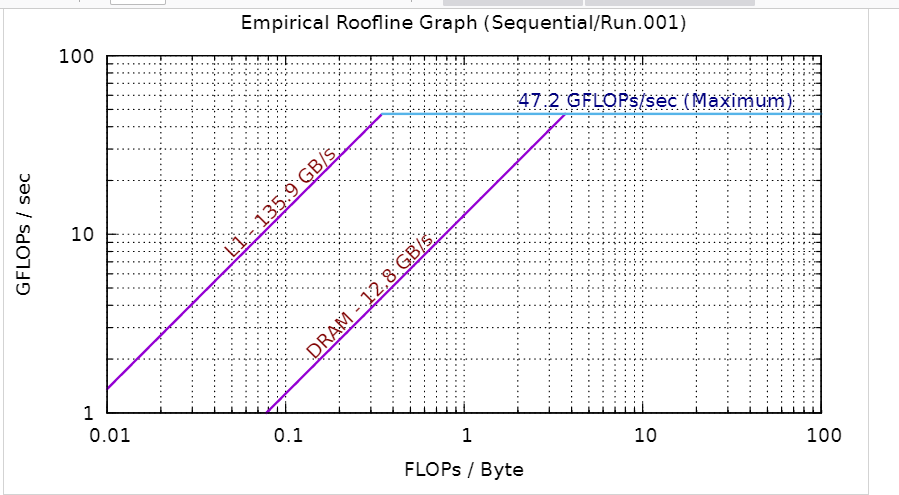
\includegraphics[width=10cm]{roofline-graph.png}
    \end{center}
    The maximal compute performance is $47.2$ GFlops per second (Very closed to mixed AVX2 with FMA3 SIMDs). The L1 is $135.9$ GB/s, the same as we observed from the homegrown benchmark. The L2 Cache bandwidth is gone under the eyes of this profiler or unknown reasons. 
    \\
    They are very similiar to the measurements above. The DRAM bandwidth is the same as results from the ``amath583/bandwidth'' docker run. 
    \\
    Back in the question 7, I assume the usage of both AVX2 with the FMA3 SIMDs, and gotten the maximal Flops throghput to be 51.6, which is the closest to what we had for the roofline in the graph computed via docker. 

\subsection*{Question 10}
    Referring to the figures about how data are stored in memory, what is it about the best performing pair of loops that is so advantageous?
    \\[1.1em]
    This is the verbatim of the out put from executing ``mmult.exe'': 
    \begin{lstlisting}
  N    GF/s ijk    GF/s ikj    GF/s jik    GF/s jki    GF/s kij    GF/s kji
  8     4.84614     4.15383     3.48922     2.72595     4.84614     3.11537
  16     3.87691     4.81272     3.47186     3.00795      4.9846     3.92047
 32     2.99043     4.97858     2.74576     3.87223     5.09045     4.67062
 64     2.33768     5.03899     2.33167     2.55498     4.95638     2.83443
128     1.71237     4.71744     1.69354     1.49195     4.64628     1.44109
256     1.14627     4.61373     1.22828     0.39231     4.80389    0.398308
    \end{lstlisting}
    The ikj and kij ordering performs the best. Observe that, the the most inner loop is \textbf{both iterating on the index} $j$. The expression $C(i, j) += A(i, k) * B(k, j)$, where the fastest interating index $j$ is running over the columns of $C$, and columns of $B$. The key here is that, running over the same column in the inner loop increases the memory locality beacuse the underlying storage of the matrix is row major, and it takes the form of ``vector$<$double$>$'', and we indexed it using ``[m*i + j]''. Notice that, incrementing on ``j'' will give us sequential access to the data. Increasing the memory locality of this numerical algorithm. Here is a graph, and we imagine how the indexing goes along the memory direction when the innerest loop is iterating through index ``j'' (stays on the same rows of the matrix $C, B$ and goes from the top to the bottom)
    \begin{center}
        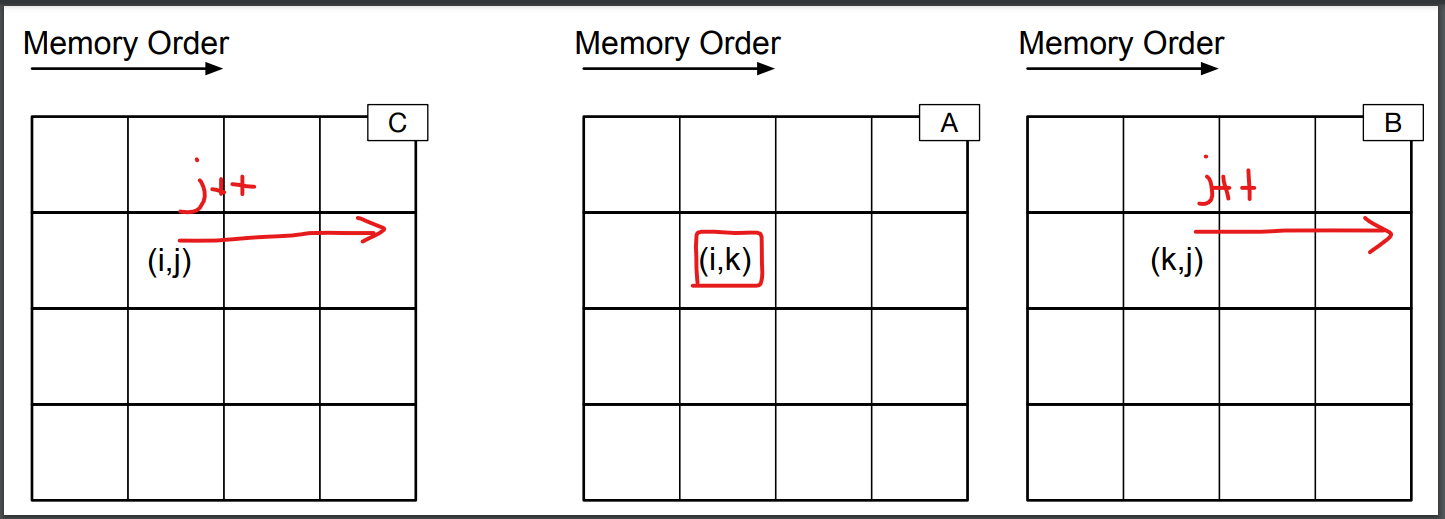
\includegraphics[width=10cm]{bestloop-ordering.png}
    \end{center}
\subsection*{Question 11}
    What will the data access pattern be when we are executing ``mult\_trans" in i,j,k order?  What data are accessed in each if the matrices at step (i,j,k) and what data are accessed at step (i, j, k+1)? Are these accesses advantageous in any way?
    \\[1.1em]
    The expression for multiplying $AB^T$ is: $C(i, j) \mathrel{{+}{=}} A(i, k) * B(j, k)$. And take notice, the inner forloop controls index $k$, and it sweeps through the $i$ th row of $A$ and the $j$ th row of $B$, from top to bottom, in a sequential manner. 
    \\[1.1em]
    This is very good because the fastest going loop is going through columns of $A,B$ and the second fastest loop is going through the row of $A, B$, in addition, $C$ is not indexed by the fastest index $k$, this maximizes the memory locality of this algorithm. 
\subsection*{Question 12}
    Referring again to how data are stored in memory, explain why hoisting  ``C(i,j)" out of the inner loop is so beneficial in mult\_trans with the ``ijk" loop ordering.
    \begin{center}
        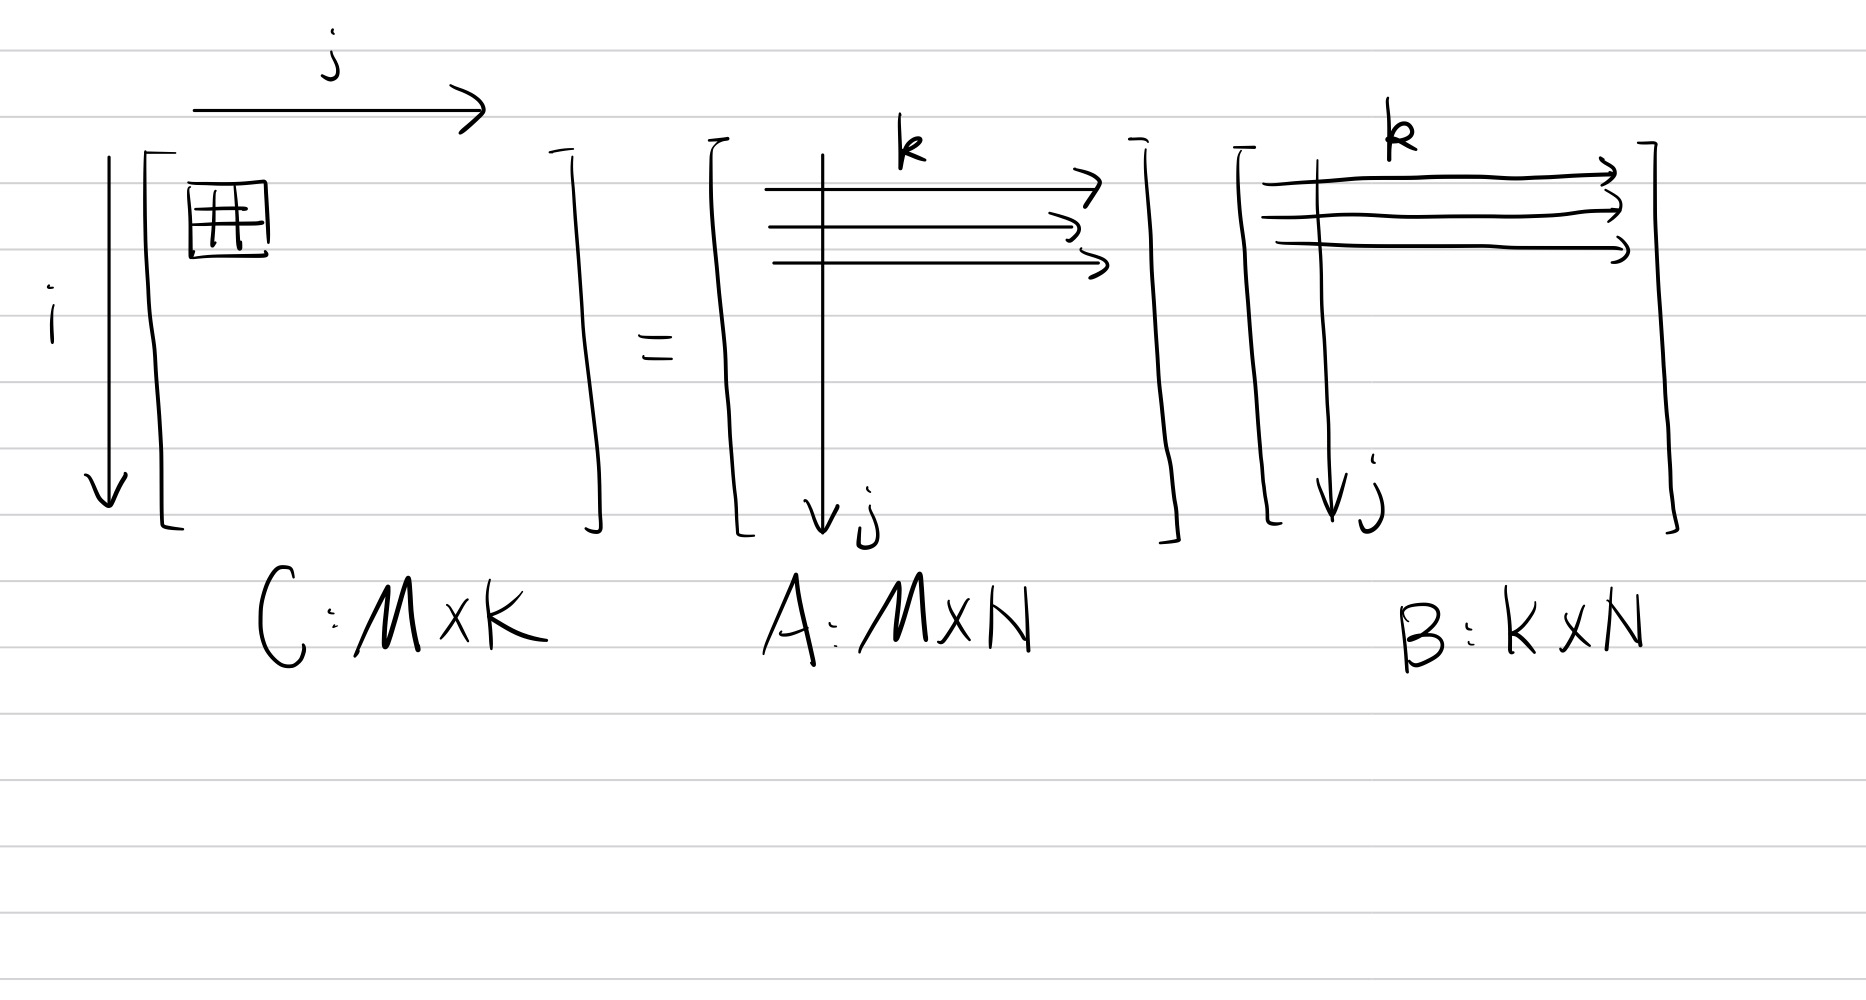
\includegraphics[width=10cm]{loop-hoist-illustrate.png}
    \end{center}
    The fastest running index ``k'' will sweep through several loops at the same time, and they will all be present with the same address space in the memory, take advantage of sequential read and increasing the speeod of the cache and compiler optimization. While the slower running index move on a larger chunks of address space. 
    \\[1.1em]
    The hoisting allows the compiler to optimize and vectorized the accumlations of all the multiply adds. 

\subsection*{Question 13}
    What optimization is applied in going from ``mult\_2`` to ``mult\_3``?
    \\[1.1em]
    Blocks of 32 by 32 is introduced in addition of tiling of 2 by 2 are used for each of the blocks. 
    \\[1.1em]
    This enables the compiler to infer more on optimizations for the cache, and the use of SMID. This also incrase the memory locality because of the usage of 32 by 32 blocks.

\subsection*{Question 14}
    How does your maximum achieved performance for ``mult`` (any version) compare to what bandwidth and roofline predicted?

\subsection*{Question 15}
    Which variant of blurring function between struct of arrays and array of structs gives the better performance? Explain what about the data layout and access pattern would result in better performance.
    \\
    Running on ``julia.bmp''
    \begin{lstlisting}
SOA inner   SOA outer   AOS inner   AOS outer   Ten inner   Ten outer
31           5           5          14          31           4
    \end{lstlisting}
    Running on ``med\_julia.bmp''
    \begin{lstlisting}
SOA inner   SOA outer   AOS inner   AOS outer   Ten inner   Ten outer
505          83          86         268         574          96
    \end{lstlisting}
    Running on ``large\_julia.bmp''
    \begin{lstlisting}
SOA inner   SOA outer   AOS inner   AOS outer   Ten inner   Ten outer
2244         371         353        1086        9592         384
    \end{lstlisting}
    The performance of SOA outer and AOS inner is similar. The SOA outer has color as the outter most for loop, and in that case, filter of the same color, stored in vector are read. However, is slower because the memory each color are no sequentially pact together. The AOS inner mitigate the jumps between each color by packing array of size 3 together into one color. Hence, when interating 3 colors inside the forloop, the memory locality is maximized and the reading of each of the pixels are sequenal as we iterate through the vector of pixels. 
    \\[1.1em]
    SOA inner is definitely worse because it jumps between different colors of filter, and they are $N*N$ bytes apart from each other in the memory. Compare to AOS, where the it jumps between different pixels in the inner forloop, and the distance between them are 3 bytes. 
    \\[1.1em]
    Therefore, the speed of AOS is faster than SOA. 

\subsection*{Question 16}
    Which variant of the blurring function has the best performance overall? Explain, taking into account not only the data layout and access pattern but also the accessor function.
    \\[1.1em]
    AOS inner has the best performance. Because the inner loop jumps between different color, which are right next to each other in the array inside of the vector, and the outter loops jumps between different pixels, which is also pack sequentially in the vector. 

\subsection*{Logs}
    \subsection*{mut\_0.log}
        \begin{lstlisting}
    N    GF/s ijk    GF/s ikj    GF/s jik    GF/s jki    GF/s kij    GF/s kji
    8     4.36152     3.79263     3.48922     2.02862     3.79263     2.29554
   16     3.81335     4.74724     3.48922     3.06072      4.9846     3.89857
   32     2.98059     4.84546     2.72102     3.83941     5.03389     4.44167
   64     2.30793     4.82457     2.30208      2.5195     5.01115      2.8256
  128     1.68691     4.66639     1.66477      1.4626     4.61643     1.44592
  256     1.19385     4.75234     1.20752     0.39688     4.80389    0.393076 
        \end{lstlisting}
    \subsection*{mult\_1.log}
        \begin{lstlisting}
    N    GF/s ijk    GF/s ikj    GF/s jik    GF/s jki    GF/s kij    GF/s kji
    8     7.93004     4.15383     3.48922     2.72595     4.84614     3.11537
   16     15.8601     4.74724     3.37123     2.84834     4.68351     3.32307
   32     24.4892     4.97858     2.72102     3.85575     5.06202     4.44167
   64     19.2983     5.01115     2.32569     2.55498     5.01115     2.90711
  128     10.9993     4.70714     1.67642     1.49299     4.71744     1.45667
  256      6.0508     4.78314     1.22016     0.39688     4.81433    0.394828     
        \end{lstlisting}
    \subsection*{mult\_2.log}
        \begin{lstlisting}
    N      mult_0      mult_1      mult_2      mult_3     mul_t_0     mul_t_1     mul_t_2     mul_t_3
    8     3.48922      3.6346     8.72305     9.69227     2.72595      5.4519     9.69227     14.5384
   16     3.45467     3.57869     9.18215     18.3643     3.38759     4.10496     9.30458     25.8461
   32     2.69673     2.77095     8.38982     25.8886     2.75411     3.02034     8.38982     32.3607
   64     2.31974      2.5195      6.9238     19.7178     2.29625     2.91646     7.49602      20.156
  128     1.71101      1.9581     7.04533     10.7794      1.9815     2.14089     6.63345     11.1127
  256     1.34708     1.59323     6.23829     5.82788     1.84089     1.91078      6.9206     6.20334     
        \end{lstlisting}
    \subsection*{mmult\_ps3.log}
        \begin{lstlisting}
    N      mult_0      mult_1      mult_2      mult_3     mul_t_0     mul_t_1     mul_t_2     mul_t_3
    8     3.48922      3.6346     8.72305     7.26921     4.84614     4.59108     9.69227     14.5384
   16     3.50675     3.57869     9.18215     8.40776     3.87691     4.12925     9.30458     25.8461
   32     2.77095     2.80527     8.54812     8.46823     2.95147     3.02034     8.38982     32.3607
   64     2.31974     2.52651     6.87135     8.39832     2.33768     2.96411       7.622     21.0934
  128     1.71373     1.98515     7.18624       7.926      2.0036     2.14301     7.23447     11.5287
  256     1.33329     1.61885     6.69061     7.16697     1.86257     1.91243      7.0082     6.20334     
        \end{lstlisting}
    \textbf{Note}: For consistency, all benchmark are run with the power of my laptop on, with maximal performance setting. 


\end{document}
